\chapter{Future implications} \label{ch14}
This chapter considers future implications of the final system described in chapter \ref{ch10}. The Fourier transform is a rather old and well-known method of frequency analysis, and the STFT provides a fine method of representing and analysing a signal in both time and frequency. However, the relation between the resolutions of time and frequencies in the STFT is lower bounded due to Heisenberg's uncertainty principle as described in theorem \ref{theo:Heisenberg}. The wavelet transform is a rather new and superior transform in signal processing compared to the Fourier transform.
\\ \\
Even though a window with a certain width that satisfies the relation $\sigma_t^2 \sigma_\omega^2 = \frac{1}{4}$ is chosen for the STFT, the width of the window cannot be changed during the analysis, which means that the Fourier transform is unsuitable to describe signals with both low and high frequencies. The wavelet transform is a different kind of transform, which is used to gain localized information in both frequency and time domains. While the Fourier transform converts a signal between the time and frequency domains, the coefficients of the wavelet transform represent details of the signal at different scale levels and their corresponding temporal location.
\begin{figure}[H]
\hspace*{-0.7cm}
\centering
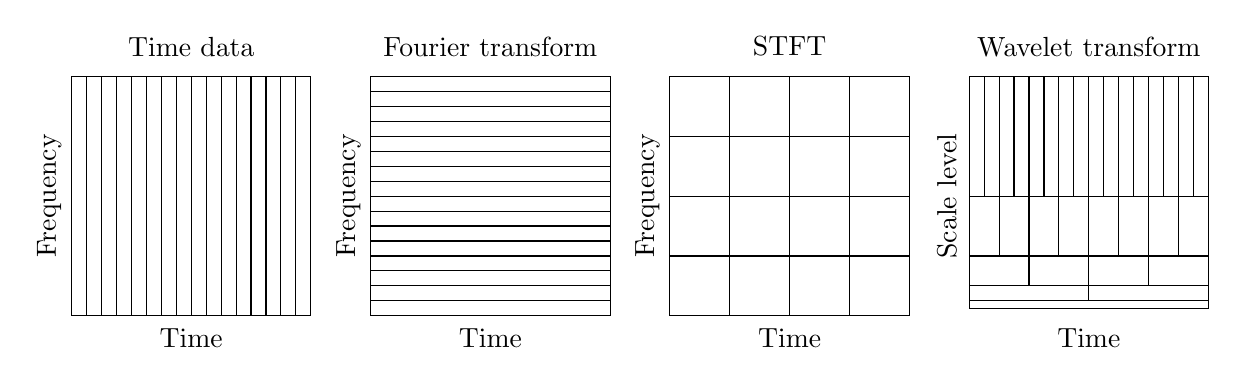
\begin{tikzpicture}[scale = 0.19]
\draw (0,0) rectangle (16,16);
\foreach \x in {0,...,16}
	\draw (\x,0) -- (\x,16);
\node[rotate=90] at (-1.5,8) {Frequency};
\node at (8,18) {Time data};
\node at (8,-1.5) {Time};

\draw (20,0) rectangle (36,16);
\foreach \y in {0,...,16}
	\draw (20,\y) -- (36,\y);
\node[rotate=90] at (18.5,8) {Frequency};
\node at (28,18) {Fourier transform};
\node at (28,-1.5) {Time};

\draw (40,0) rectangle (56,16);
\foreach \y in {4,8,12}
	\draw (40,\y) -- (56,\y);
\foreach \x in {44,48,52}
	\draw (\x,0) -- (\x,16);
\node[rotate=90] at (38.5,8) {Frequency};
\node at (48,18) {STFT};
\node at (48,-1.5) {Time};

\draw (60,0.5) rectangle (76,16);
\foreach \y in {1,2,4,8}
	\draw (60,\y) -- (76,\y);
\foreach \x in {68}
	\draw (\x,1) -- (\x,16);
\foreach \x in {64,72}
	\draw (\x,2) -- (\x,16);	
\foreach \x in {62,66,70,74}
	\draw (\x,4) -- (\x,16);	
\foreach \x in {61,63,65,67,69,71,73,75}
	\draw (\x,8) -- (\x,16);		
	
\node[rotate=90] at (58.5,8) {Scale level};
\node at (68,18) {Wavelet transform};
\node at (68,-1.5) {Time};

\end{tikzpicture}
\caption{Comparisons of temporal and frequency locations in the Fourier and wavelet transforms.}
\label{fig:wave}
\end{figure}

This is summarized by figure \ref{fig:wave}, which shows 4 \textit{Heisenberg boxes}, where the area of each cell in each box are\trine{ikke sandt for den sidste jo} similar \cite{page 410, Wang}. The first box shows the signal in time with full time resolution but no frequency resolution; the second box shows the frequency spectrum achieved by the Fourier transform of the signal with full frequency resolution but no time resolution; the third box shows the STFT of the signal with a fixed window size and with equally (but not arbitrarily) good resolutions in time and frequency; and finally, the fourth box shows the wavelet transform of the signal with varying scale levels and their corresponding time resolutions. At a low scale level the window is wide, which gives a good frequency resolution but poor time resolution, and at a high scale level the window is narrow, which conversely gives poor frequency resolution but good time resolution. Furthermore, the area of each cell in the boxes for the STFT and the wavelet transform are determined by the width of the window and the particular wavelet being used, respectively \cite{pages 409-410, Wang} \cite{page 43-44, wave_tut}.

\section{Definition of wavelets}
Wavelet theory provides a way of constructing orthonormal bases in the space $\mathcal{L}^2(\mathbb{R})$. A wavelet system is scaled and translated versions of a fixed function. For an orthonormal basis $\{\textbf{e}_k\}$ of $\mathcal{L}^2(\mathbb{R})$ all functions $f \in \mathcal{L}^2(\mathbb{R})$ have an expansion
\begin{align*}
f = \sum_{k\in\mathbb{Z}}^\infty \langle f, \textbf{e}_k \rangle \textbf{e}_k.
\end{align*}

The index set of the sum is generally infinite but in order for the representation to be of practical use, the functions $f$ must be able to be approximated well by finite partial sums \cite{page 160, FSE2010}.

\begin{definition}[Wavelet]
Let $\psi \in \mathcal{L}^2(\mathbb{R})$.
\begin{enumerate}
\item For $j,k \in \mathbb{Z}$, define the function $\psi_{j,k}$ by
\begin{align*}
\psi_{j,k}(t) = 2^{j/2} \psi(2^jt-k), \quad t \in \mathbb{R}.
\end{align*}
\item The function $\psi$ is called a wavelet if the functions $\{\psi_{j,k}\}_{j,k\in\mathbb{Z}}$ form an orthonormal basis for $\mathcal{L}^2(\mathbb{R})$.
\end{enumerate}
\end{definition}

Therefore, $\psi_{j,k}$ is a dilation and translation as defined in definition \ref{def:TMD} and may be written in terms of the translation operator $T_k$ and the dilation operator $D$ as \cite{page 160, FSE2010}
\begin{align*}
\psi_{j,k} = D^j T_k \psi, \quad j,k \in \mathbb{Z}.
\end{align*}

A simple wavelet is the Haar wavelet.

\begin{definition}[Haar Wavelet] \label{HaarWave}
The \textit{Haar function} is defined by
\begin{align*}
\psi(t) =
\begin{cases}
1 \quad &\textnormal{if } 0 \leq t < \frac{1}{2} \\
-1 \quad &\textnormal{if } \frac{1}{2} \leq t < 1 \\
0 \quad &\textnormal{otherwise}
\end{cases}
\end{align*}
\end{definition}

%The proof that the functions $\{\psi_{j,k}\}_{j,k\in\mathbb{Z}}$ constitute an orthonormal basis for $\mathcal{L}^2$ is quite technical and will therefore be skipped as the purpose of this chapter is merely to introduce and apply wavelet analysis as an alternative to the Fourier transform \cite{page 161, FSE2010} \martin{Overvej dette. \textregistered}.
%\\ \\
The wavelet $\psi(t)$ is usually compactly supported, which means that $\psi(t) \neq 0$ only inside a bounded interval $a < t < b$. Furthermore, $\psi(t) \in \mathcal{L}^1$ has zero mean, which means that it takes both positive and negative values:
\begin{align*}
\int_{-\infty}^\infty \psi(t) dt = 0.
\end{align*}

Therefore, since a wavelet is nonzero only within a finite range and the mean is zero, then $\psi(t)$ has the form of a wave, which is the reason why $\psi(t)$ is called a wavelet \cite{page 411, Wang}. The Haar wavelet is discontinuous at $t = 0, \frac{1}{2}, 1$. Examples of other wavelets that are continuous are the Shannon, Mortlet, and Marr wavelets \cite{page 417-420, Wang}.
\\ \\
The following definition is the background for a main theorem of this section \cite{page 170, FSE2010}.

\begin{definition}[Vanishing moments]
Let $N \in \mathbb{N}$. A function $\psi$ has $N$ vanishing moments if
\begin{align*}
\int_{-\infty}^\infty x^\ell \psi(x) dx = 0 \quad for \quad \ell = 0, 1, \dots, N-1.
\end{align*}
\end{definition}

A relevant wavelet function is the Daubechies' wavelet of degree $N$, which has $N$ vanishing moments and is supported on $[0,2N-1]$. The Haar wavelet defined in definition \ref{HaarWave} is a Daubechies' wavelet of degree $1$ \cite{page 174, FSE2010}. If the wavelet $\psi$ has a large number of vanishing moments, the following result shows that only relatively few coefficients $\langle f, \psi_{j,k} \rangle$ will be large and therefore only a small number of wavelets are needed in the expansion.

\begin{theorem}[Decay of wavelet coefficients]
Assume that the function $\psi \in \mathcal{L}^2(\mathbb{R})$ is compactly supported and has $N$ vanishing moments. Then, for any $N$ times differentiable function $f \in \mathcal{L}^2(\mathbb{R})$ for which the $N$'th derivative $f^{(N)}$ is bounded, there exists a constant $C > 0$ such that
\begin{align} \label{eq:decay_wave_coeff}
|\langle f, \psi_{j,k} \rangle| \leq C 2^{-jN} 2^{-j/2}, \quad \forall \ j \geq 1, \quad k \in \mathbb{Z}.
\end{align}
\end{theorem}

\eqref{eq:decay_wave_coeff} suggests that a high number of vanishing moments $N$ implies that the numbers $\langle f, \psi_{j,k} \rangle$ decay quickly as $j \to \infty$. Therefore, the higher the number of vanishing moments a wavelet has, the fewer coefficients $\{ \langle f, \psi_{j,k} \rangle \}_{j\in\mathbb{N},k\in\mathbb{Z}}$ are needed in the expansion \cite{page 170, FSE2010}.
\\ \\
This fact is widely used in different areas of signal processing. In images, small coefficients signify constant intensities, while large coefficients signify edges. Performing wavelet analysis by using a wavelet with many vanishing moments means that many of the coefficients can be discarded by thresholding, which is an efficient compression \cite{page 174, FSE2010}.
\\ \\
Similarly, noise from audio signals like the ones used in this project may be reduced by removing some of the coefficients \cite{page 175, FSE2010}.
\\ \\
Apart from a different type of transform, the final system could also be using different types of filters as described in the discussion in chapter \ref{ch12}. Apart from the methods being used in the system, future implications also involve designing an app capable of performing the analysis, recognizing the exact frequencies in a rather noisy environment at certain times with respect to a given number of beats per minute, and finally showing the result in a staff system, which the musician may edit, save and print. Naturally, such system is highly desired by musicians all over the world, and big companies designing music notation softwares (such as the Sibelius software from Avid) are obviously working hard to design this kind of system. Therefore, the need for and range of future implications of the system described in this project are obviously huge.